\chapter{Introducción específica} % Main chapter title

\label{Chapter2}

%----------------------------------------------------------------------------------------
%	SECTION 1
%----------------------------------------------------------------------------------------
En este capítulo se profundiza en conceptos de negocio que son importantes comprender para el desarrollo del trabajo. Adicionalmente se detallan los requerimientos y se brinda más detalle sobre los modelos de inteligencia artificial usados en la solución.

\section{Variables y reglas de negocio}
\label{sec:Negocio}

El Banco de Crédito del Perú es el banco más grande de su país con más de 11 millones de clientes y más de 17 mil empleados. Cuenta con diversas áreas de negocio repartidas según canales de atención, segmentos de clientes o productos. Por ejemplo, existen equipos de trabajo para canales alternativos como cajeros, otros para segmentos de clientes afluentes, y equipos para productos hipotecarios o de medios de pago, entre muchos otros. Cada uno de estos tiene analistas de negocio que se encargan de gestionar campañas comerciales o proyectos, muchos de los cuales exigen comunicaciones a los clientes. El email es uno de los primeros canales de comunicación que se eligen ya que no implica uso del presupuesto de área y es relativamente fácil de gestionar. Sin embargo, la mayoría de los pedidos de correos son derivados a un solo equipo de diseño, quien muchas veces debe priorizar y postergar algunos pedidos por falta de capacidad.

El equipo de diseño desarrolla los emails en base a \textit{briefs}. En el caso de campañas grandes que exigen varios canales de comunicación y una estrategia más compleja, se tienen \textit{briefs} más extensos. Pero en general, para correos tácticos, se utiliza un \textit{mini-brief} que incluye estas preguntas:

\begin{enumerate}
    \item Objetivo de la campaña:
    \item ¿Quién es nuestro público objetivo?
    \item ¿Qué queremos decirles?
    \item ¿A qué segmentos va dirigido? Si incluye ENALTA, confirmar la firma de quién irá en el mail.
    \item Tipo de Piezas y mandatorios
\end{enumerate}

Las tres primeras preguntas ayudan a dar contexto sobre qué se quiere lograr con la comunicación, cómo adaptarla según el público al que va dirigida y detalla el contenido del email. La cuarta pregunta pide especificar el segmento del cliente.

Dentro del banco, existen diferentes segmentos de clientes personas naturales que se definen principalmente en base a los ingresos y patrimonio de los estos. De menos a más ingresos, estos son los segmentos: 
\begin{itemize}
    \item Consumo
    \item Banca Exclusiva (BEX)
    \item Enalta
    \item Privada
\end{itemize}

Cada segmento tiene colores y diseños de emails ligeramente diferentes. En específico, Enalta y Privada tienen incluso sus propios logos. Adicionalmente, los cierres de los correos cambian. En Consumo, el cierre es más general y se derivan las consultas a canales de atención masivos. Para el resto de los segmentos, los cierres derivan las consultas a los funcionarios asignados a cada cliente en específico, por lo que en el código HTML se incluyen campos personalizables para estos casos. Para el alcance del presente trabajo solo se están considerando los segmentos Comsumo y BEX, ya que abarcan la mayoría de clientes. 

En las figuras~\ref{fig:EjConsumo} y~\ref{fig:EjBEX} se pueden visualizar ejemplos de las variantes de emails de una misma campaña para estos dos segmentos. Adicionalmente, también podemos ver un análisis inicial que se ha realizado de las partes que componen un correo, lo cual será crucial para el desarrollo de la solución. Como se puede notar, La cabecera y el cierre son los que más variaciones tienen entre Consumo y BEX. Además, a veces también se presentan cambios en el color del texto para resaltar frases importantes.

Otra sección del correo que es importante considerar son los Términos y Condiciones (T\&C) y los legales. Los T\&C son opcionales y los analistas de negocio los tienen que compartir textualmente en el \textit{brief}. Estos se incluyen sin ninguna modificación en el email, ya que han sido revisados previamente por el área de legal. Adicionalmente, existe un texto genérico que se incluye en todos los emails del banco (los dos últimos párrafos). Este legal genérico no es necesario mencionarlo en el \textit{brief} ya que el equipo de diseño siempre lo incluye en los correos como parte de los lineamientos que tiene. 

Por último, para comunicaciones de productos que tienen asociadas tasas, es necesario incluir tasas referenciales en el legal. La tasa especificada puede ser tasa de costo efectiva anual (TCEA) para productos activos (aquellos que involucran que el banco preste dinero al cliente), o tasa de rendimiento efectiva anual (TREA) para productos pasivos (aquellos en los que el cliente deja su dinero en custodia del banco). Tanto la tasa como su descripción también deben ser brindadas por el analista de negocios en el \textit{brief}.

\cleardoublepage
\begin{figure}[!htpb]
     \centering
     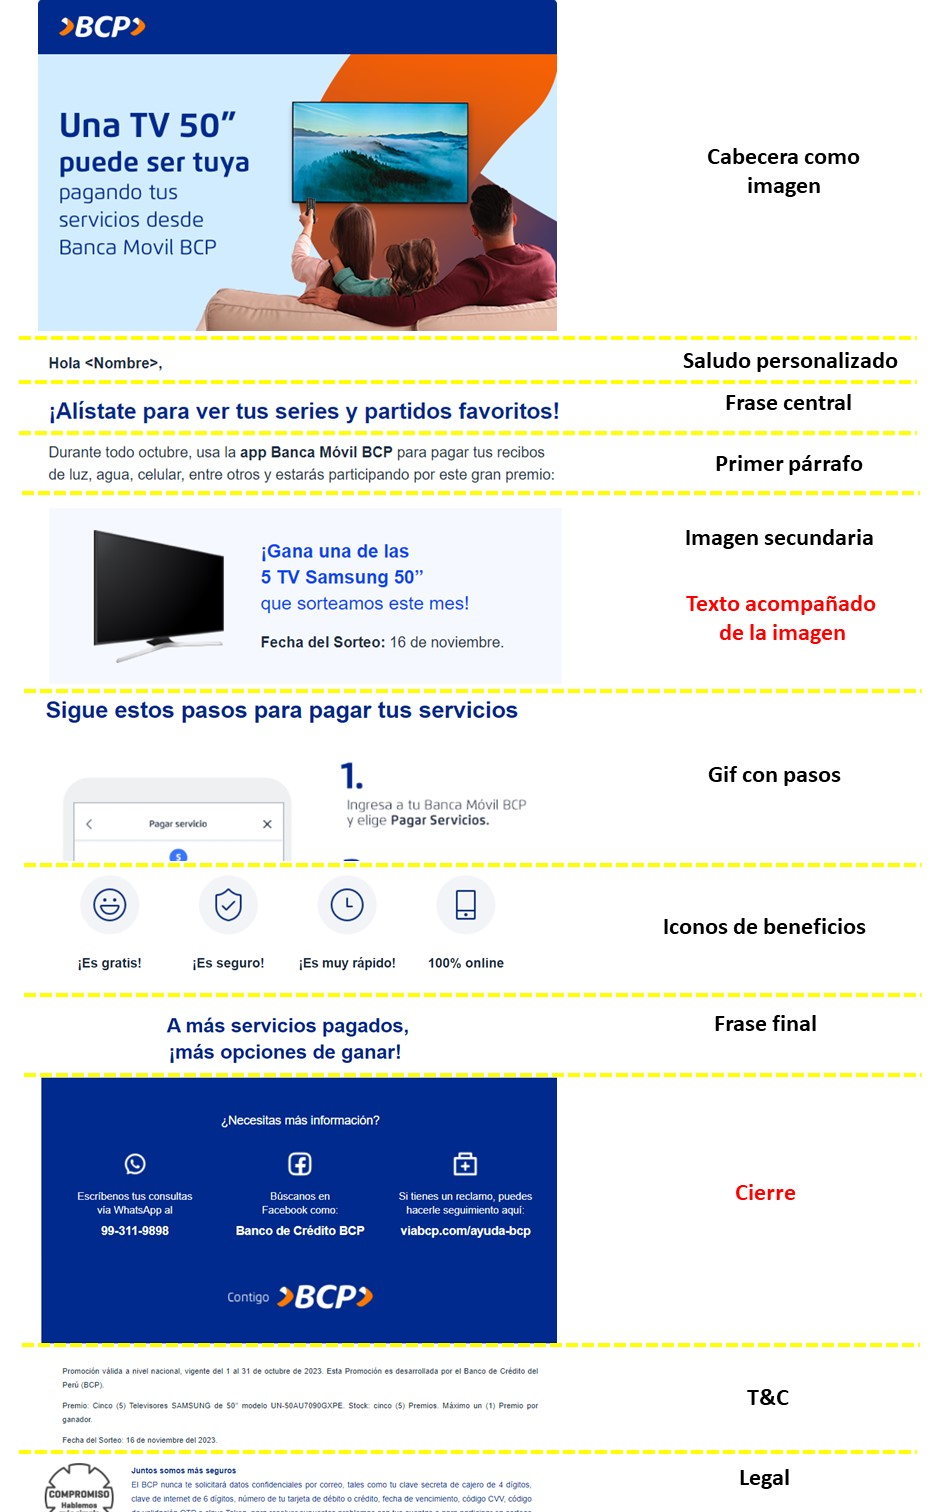
\includegraphics[width=0.8\textwidth]{./Figures/ejemplo_Consumo}
    \caption{Ejemplo de email para Consumo}
    \label{fig:EjConsumo}
\end{figure}

\begin{figure}[!htpb]
     \centering
     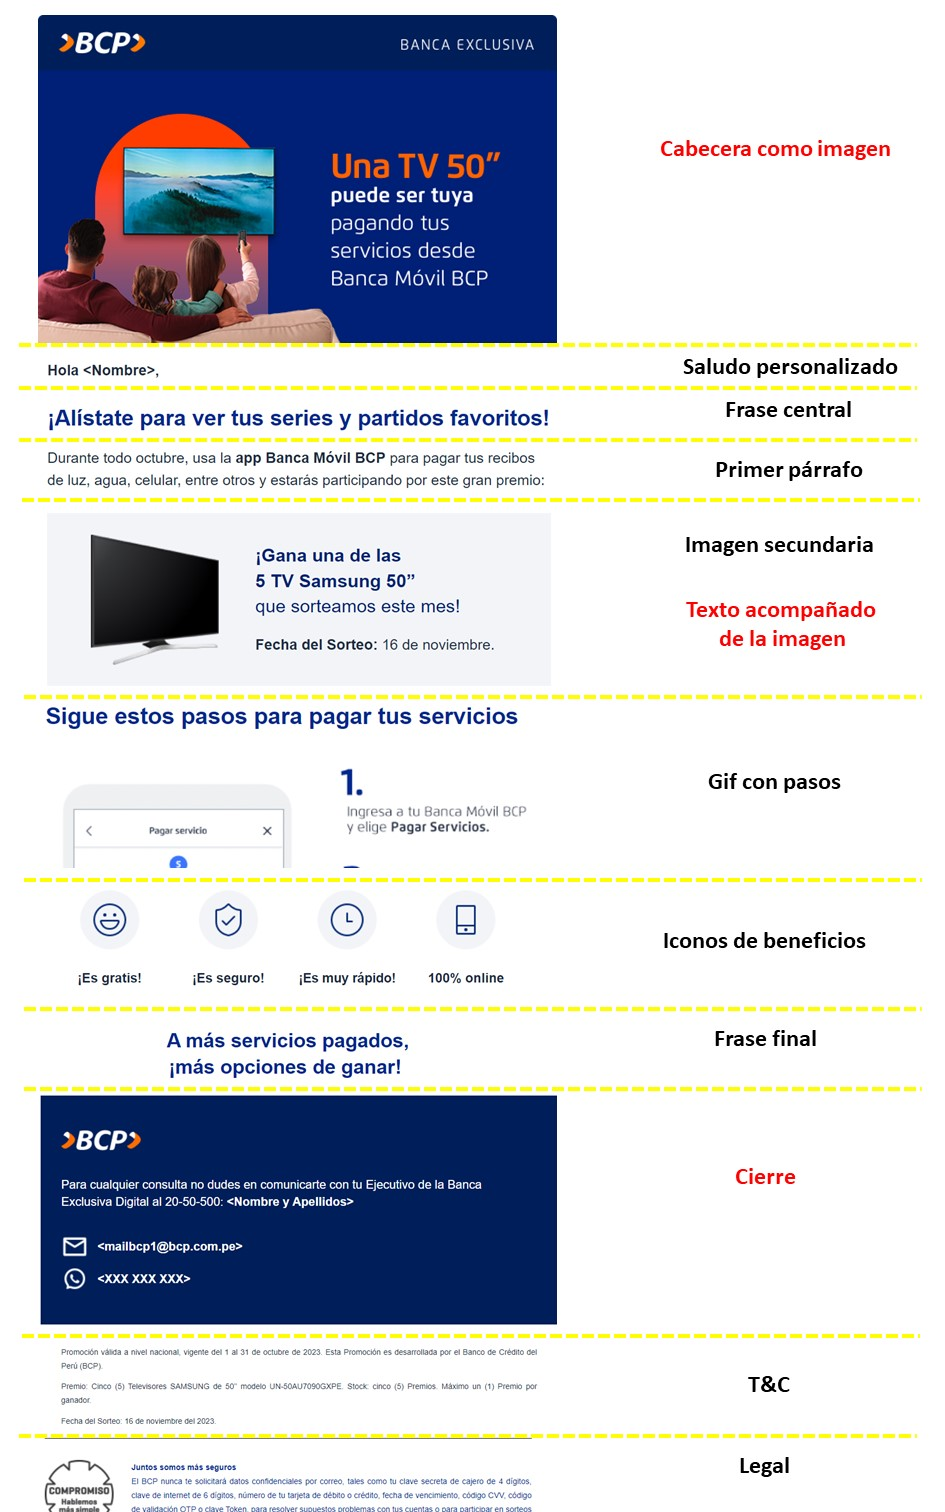
\includegraphics[width=0.8\textwidth]{./Figures/ejemplo_BEX}
     \caption{Ejemplo de email para BEX}
     \label{fig:EjBEX}
\end{figure}


\section{Requerimientos}

Los requerimientos que se han considerado al momento de desarrollar el presente trabajo son los siguientes:

\begin{enumerate}
	\item Requerimientos funcionales
		\begin{enumerate}
			\item El sistema debe generar un boceto de email según lo información brindada en un \textit{brief} que incluye: 1) Objetivo de la campaña 2) Público objetivo 3) Mensaje que se desea comunicar.
			\item El formato final del proceso es un archivo index.html con una carpeta ``img"  que contenga las imágenes necesarias para el mail. Este formato es compatible con Adobe Campaign.
			\item Se debe generar un output intermedio que permita al usuario revisar el contenido del email antes de su versión final.
			\item El email generado debe cumplir con los lineamientos de diseño de correos de la empresa, considerando que el formato cambia según los segmentos de clientes.
		\end{enumerate}
	\item Requerimientos de confidencialidad y seguridad
		\begin{enumerate}
			\item La información de la empresa brindada para entrenar el modelo no debe ser compartida con terceras empresas.
			\item La información que se comparte al modelo mediante los \textit{briefs} no debe contener datos de alta criticidad de clientes o personas (número de documento, nombres, datos de contacto, entre otros).
		\end{enumerate}
	\item Requerimientos de la interfaz (opcional)
		\begin{enumerate}
			\item El modelo debe poder ser utilizado por usuarios no técnicos pertenecientes a equipos de diseño y marketing.
		\end{enumerate}
\end{enumerate}

\section{Modelos de generación de texto utilizados}

El Procesamiento del Lenguaje Natural (PLN) es un campo de la inteligencia artificial que se encarga de la interacción entre las computadoras y el lenguaje humano. Este campo abarca el desarrollo de algoritmos y sistemas que permiten a las máquinas comprender, interpretar y generar lenguaje humano de manera efectiva, facilitando aplicaciones como la traducción automática, el análisis de sentimientos, los chatbots y la síntesis de texto \cite{jurafsky2021}.

Los Modelos de Lenguaje a Gran Escala (LLMs, por sus siglas en inglés) son modelos de aprendizaje profundo entrenados en grandes cantidades de texto para predecir la probabilidad de secuencias de palabras. Se les llama "grandes" por la enorme cantidad de parámetros que manejan, lo cual les permite captar complejidades y matices del lenguaje natural \cite{vaswani2017}.

Estos modelos han sido entrenados utilizando técnicas de pre-entrenamiento en grandes corpus de texto, lo que les permite aprender patrones y estructuras del lenguaje. Utilizan tokens, que son unidades básicas de texto (como palabras o subpalabras), para procesar y generar lenguaje. Actualmente, los LLMs se utilizan para una variedad de tareas como la generación de texto, la traducción automática, la respuesta a preguntas y la síntesis de texto \cite{vaswani2017}.

Entre los LLMs más destacados disponibles actualmente se encuentran GPT-4, Claude, GPT-3.5, Vicuna, y LLaMA, entre otros. Algunos de estos modelos son de código abierto, como Vicuna y LLaMA, mientras que otros son privados, como GPT-4. Un estudio reciente comparó estos modelos utilizando tanto jueces humanos como las propias LLMs para determinar cuál es mejor en diversas tareas. En este estudio, GPT-4 fue uno de los modelos ganadores, mostrando un rendimiento superior en varias métricas \cite{zheng2023judging}. La figura a continuación muestra la tasa de victorias promedio de nueve modelos bajo diferentes jueces en Chatbot Arena:

\begin{figure}[h]
  \centering
  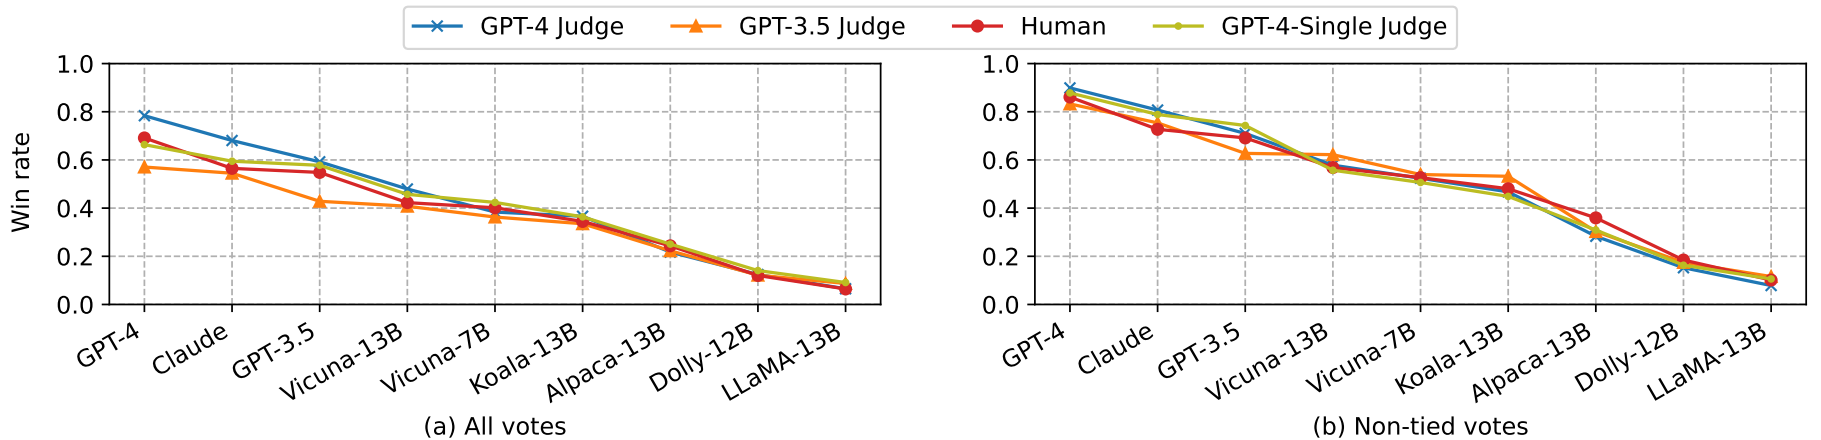
\includegraphics[width=\linewidth]{./Figures/comparacion_LLMs.png}
  \caption{Tasa promedio de victorias de nueve modelos bajo diferentes jueces. Primer gráfico considerando todos los votos y segundo, solo los votos sin empates\cite{zheng2023judging}.}
\end{figure}

Varias LLMs privadas están disponibles para su uso mediante API. Por ejemplo, OpenAI ofrece una API que permite acceder a modelos como GPT-4o, GPT-4 y GPT-3, entre otros. Estas API ofrecen funcionalidades como el modo JSON para estructurar las respuestas. El uso de estas API se cobra en función de los tokens de entrada y salida procesados. En nuestro proyecto, decidimos usar GPT-4o, ya que es un modelo más reciente que GPT-4 y resulta más económico \cite{openai}.

LangChain es un marco de trabajo diseñado para facilitar el desarrollo de aplicaciones que utilizan LLMs. Es útil porque proporciona herramientas y abstracciones para conectar modelos de lenguaje con otras fuentes de datos y sistemas, permitiendo la creación de flujos de trabajo complejos y personalizados. Las cadenas en LangChain funcionan conectando diferentes componentes que procesan y transforman datos en pasos secuenciales \cite{langchain}.

Además, mediante LangChain también se pueden crear agentes de inteligencia artificial. Un agente AI es un sistema que puede percibir su entorno y tomar acciones para alcanzar objetivos específicos. En LangChain, se pueden definir herramientas (tools) que los agentes pueden utilizar para ejecutar funciones dentro de las aplicaciones, permitiendo una interacción más rica y compleja con los usuarios \cite{langchain}.

\section{Modelos de generación de imágenes utilizados}